\documentclass{article}

% Packages
\usepackage[utf8]{inputenc} %for modern characters
\usepackage{microtype} % for sexy kerning
\usepackage{hyperref} %for cross-referencing and urls
\usepackage{mathtools} % for math stuff
\usepackage{amssymb} % for math symbols
\usepackage{tabularx} % For making tables
\usepackage{listings} % For writing code
\usepackage{pdfpages} % For including pdfs

% Set the margins
\usepackage[scale=0.8,top=1in,bottom=1in]{geometry}

% Other Front Matter
\lstset{language=R} % Set listing language to R
\graphicspath{ {img/} } % Put all graphics in img/
\newcommand{\code}[1]{\texttt{#1}} % More readable for writing inline code.
\newcommand{\p}[1]{\paragraph{#1}} % Easier to type out for paragraph command
%\newcommand{\tab}{\hspace*{3em}} % Set tab spaces
\setlength{\parindent}{0pt} % Get rid of indents
\setcounter{tocdepth}{3} % sections, subsections and sub subsections in TOC

%%%%%%%%%%%%%%%%%%%% Begin Document %%%%%%%%%%%%%%%%%%%%
\begin{document}

% Title page and TOC
{
	\title{TMATH 390 \\ Probability and Statics for Engineers \\ NOTES}
	\author{Ben Foster\thanks{
		Institute of Technolgy, University of Washington Tacoma} \\
		\url{benf94@uw.edu}
	}
	\date{March 31, 2015}
	\maketitle
	\thispagestyle{empty} % No page number at bottom
	\begin{abstract}
	\begin{center}
		This document contains the notes from the course TMATH 390 and does not necessarily
		contain all the information provided by the instructor.
	\end{center}
	\end{abstract}
	\clearpage
	\pagenumbering{roman}
	\tableofcontents
	\clearpage
	\setcounter{page}{1}
	\pagenumbering{arabic}
}
	
\section{Data and Distributions} %%% Chapter 1 Page 1

The discipline of statistics teaches us how to make intelligent judgments and informed decisions in the presence of uncertainty and variation.

	\subsection{Populations, Samples, and Processes} %%% Section 1.1
	An investigation will typically focus on a well-defined collection of objects constituting a 
	\textbf{population} of interest. In one study, the population might consist of all gelatin capsules 
	of a particular type produced during a specified period. When desired information is available 
	for all objects in the population, we have what is called a \textbf{census}. A subset of the 
	population -- a \textbf{sample}-- is usually selected in some prescribed manner to get feedback 
	on the population.
	
	\subsection{Visual Displays for Univariate Data} %%% Section 1.2
	\p{Stem-and-Leaf Displays} These can be an effective way to organize numerical data without 
	expending much effort. It is based on separating each observation into two parts: a 
	\textbf{stem}, consisting of one or more leading digits, and a \textbf{leaf}, consisting of the 
	remaining or trailing digit(s). Example:
	\begin{table}[!htb]
	\centering
	\begin{tabular}{ l l }
		0 & 4 \\
		1 & 1345678889 \\
		2 & 1223456666777889999 \\
		3 & 0112233344555666677777888899999 \\
		4 & 111222223344445566666677788888999 \\
		5 & 00111222233455666667777888899 \\
		6 & 01111244455666778
	\end{tabular}
	\caption{Percentage binge drinkers at each of 140 colleges}
	\label{tab:binge_drinkers}
	\end{table}
	
		\subsubsection{Dotplots} 
		A dotplot is an attractive summary of numerical data when the data set is reasonably small 
		or there are relatively few distinct data values. Each observation is presented by a dot 
		above the corresponding location on a horizontal measurement scale. When a value 
		occurs more than once, there is a dot for each occurrence, and these dots are stacked 
		vertically. Example: Here is data on state-by-state appropriations for higher education as a 
		percentage of state and local tax revenue for fiscal year 2009-2010: \\
	
		\begin{center}
		\begin{tabular}{ c c c c c c c c c c }
			14.0 & 3.1 & 8.6   & 9.6   & 7.4 & 4.0 & 4.5 & 6.5 & 6.1 & 8.8 \\
			8.2   & 8.6 & 6.4   & 6.7   & 8.0 & 8.5 & 9.4 & 9.5 & 4.6 & 6.8 \\
			3.9   & 6.9 & 6.3   & 11.9 & 5.8 & 5.8 & 9.9 & 5.9 & 2.7 & 4.2 \\
			14.9 & 4.0 & 12.1 & 8.0   & 5.2 & 9.2 & 6.8 & 4.3 & 3.9 & 9.6 \\
			8.0   & 8.6 & 8.6   & 8.7   & 3.1 & 5.8 & 6.2 & 8.7 & 6.8 & 8.9 \\
		\end{tabular}
		\end{center}

		\begin{figure}[!htb]
		   \centering
		   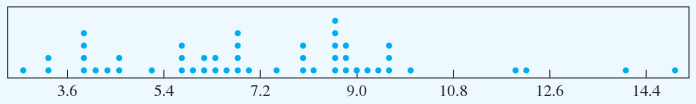
\includegraphics[width=4in]{dotplot_example.jpg} 
		   \caption{example caption}
		   \label{fig:example}
		\end{figure}
		
		\subsubsection{Histograms} 
		Some numerical data is obtained by counting to determine the value of a variable, 
		whereas other data is obtained by taking measurements. The prescription for drawing a 
		histogram is different for these two cases. \\
	
		A variable is \textbf{Discrete} if its set of possible values either is finite or else can be listed 
		in an infinite sequence. A variable is \textbf{continuous} if its possible values consist of an 
		entire interval on the number line. \\
		Consider data consisting of observations on a discrete variable $x$. The 
		\textbf{Frequency} of any particular $x$ value is the number of times that value occurs in 
		the data set. The \textbf{Relative Frequency} of a value is the fraction or proportion of time 
		the value occurs.
		\[ \text{relative frequency of a value} = \frac{\text{number of times the value occurs}}
		{\text{number of observations in the data set}} \]
		Here is an example of a histogram:
	
		\begin{table}[!htb]
		   \centering
		   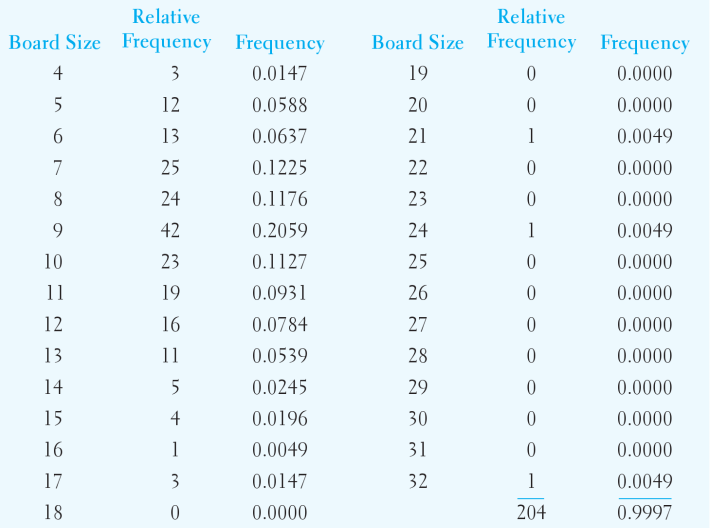
\includegraphics[width=4in]{histo_example_table.jpg} 
		   \caption{Table of board members for hospitals}
		   \label{tab:histo_table}
		\end{table}
	
		\begin{figure}[!htb]
		   \centering
		   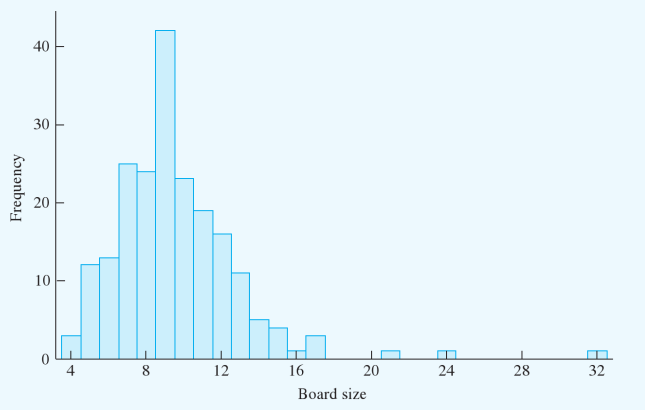
\includegraphics[width=4in]{histo_example.jpg} 
		   \caption{Example of a Histogram}
		   \label{fig:histo_example}
		\end{figure}
	
	\p{Constructing a Histogram for Continuous Data: Equal Class Widths}
	Determine the frequency and relative frequency for each class. Mark the class boundaries 
	on a horizontal measurement axis. Above each class interval, draw a rectangle whose 
	height is the corresponding relative frequency (or frequency).
	
	\p{Constructing a Histogram for Continuous Data: Unequal Class Widths}
	After determining the frequencies and relative frequencies, calculate the height of each 
	rectangle using the formula:
	\[ \text{rectangle height} = \frac{\text{relative frequency of the class}}{\text{class width}} \]
	The resulting rectangle heights are usually called \emph{densities}, and the vertical scale 
	is the \textbf{density scale}. This prescription will also work when the class widths are 
	equal.
	
		\subsubsection{Histogram Shapes}
		Histograms come in a variety of shapes. A \textbf{unimodal} histogram is one that rises to 
		a single peak and then declines. A \textbf{bimodal} histogram has two different peaks. 
		Bimodality occurs when the data set consists of observations on two quite different kinds 
		of individuals or objects. A histogram with more than two peaks is said to be 
		\textbf{multimodal}. Of course, the number of peaks may well depend on the choice of 
		class intervals, particularly with a small number of observations. \\
		
		A histogram is \textbf{symmetric} if the left half is a mirror image of the right half. A 
		unimodal histogram is \textbf{positively skewed} if the right or upper tail is stretched out 
		compared with the left or lower tail, and \textbf{negatively skewed} if the longer tail extends 
		to the left.
		
		\begin{figure}[!htb]
		   \centering
		   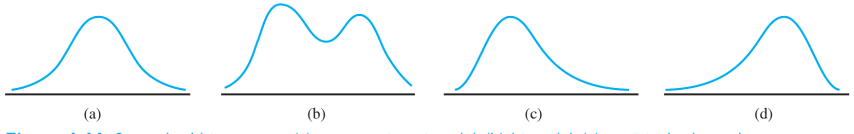
\includegraphics[width=4in]{histograms.jpg} 
		   \caption{Smoothed Histograms: (a) symmetric unimodal; (b) bimodal; (c) positively 
		   	skewed; (d) negatively skewed}
		   \label{fig:histograms}
		\end{figure}	
		
		\subsubsection{Categorical Data}
		A histogram for categorical data is often called a \textbf{bar chart}. In come cases, there 
		will be a natural ordering of classes (for example, freshman, sophomore, junior, senior), 
		whereas in other cases, the order will be arbitrary (Honda, Yamaha, Ford, etc.). A 
		\textbf{Pareto diagram} is a bar chart resulting from a quality control study in which 
		category data represents a different type of product nonconformity or production problem.
	
	\subsection{Describing Distributions} %%% Section 1.3
	In Section 1.2, we saw that a histogram could be used to describe how values of a variable $x$ 
	are distributed in a data set. In practice, a histogram is virtually always constructed from sample 
	data.
	
		\subsubsection{Continuous Distributions}
		
	
	\subsection{The Normal Distribution} %%% Section 1.4
	
	\subsection{Other Continuous Distributions} %%% Section 1.5
	
	\subsection{Several Useful Discrete Distributions} %%% Section 1.6

\clearpage
\section{Numerical Summary Measures} %%% Chapter 2 Page 61

	\subsection{Measures of Center} %%% Section 2.1
	
	\subsection{Measures of Variability} %%% Section 2.2
	
	\subsection{More Detailed Summary Quantities} %%% Section 2.3

	\subsection{Quantile Plots} %%% Section 2.4
	Constructing a Quantile plot can take a little more work than constructing a regular 
	distribution. For example, when making a Normal Quantile Plot, you would use the 
	following definition for a sample quantile: Let $x_{(1)}$ denote the smallest sample 
	observation, $x_{(2)}$ the second smallest observation,$...$, and $x_{(n)}$ the largest 
	sample observation. For $i=1,...,n, x_{(i)}$ is the $[(i-0.5/n]$th sample quantile.
	
	Therefore, to make the Normal Quantile Plot, you would use the coordinates:
	\[ \left(\left(\frac{0.5}{n}\right)\text{th quantile,} x_{(1)}\right),...,\left(\left(\frac{i-0.5}{n}\right)
	\text{th quantile,} x_{(n)}\right)\]

	The plot of this, if a true normal distribution, should fall close to a $45^\circ$ angle or a line 
	with a slope of 1 passing through the point (0,0). \\

	If you get a normal distribution that isn't standard, then you would use this:
	\[ \text{quantile for normal }(\mu , \sigma) \text{distribution} = \mu + \text{(corresponding z 
	quantile)}\sigma \]
	
	% Some bullshit about Weibull log plots.
	
	% Remember that \bar{x} is the average of the data.

\clearpage	
\section{Bivariate and Multivariate Data and Distributions} %%% Chapter 3 Page 101
Bivariate and Multivariate Data and Distributions: \\
	
A multivariate data set consists of observations made simultaneously on two or more variables. 
One important special case is that of bivariate data, in which observations on only two 
variables, $x$ and $y$  are available. We will also discuss the correlation coefficient which is a 
measure of how strongly two variables are related.
	
	\subsection{Scatterplots} %%% Section 3.1
	Scatterplots are the best way to graphically describe Bivariate data sets. In R, typing in the 
	command \code{plot(A,B)} will print out the scatter plot with A being x and B being Y where 
	as the command \code{plot(A $\sim$ B)} treats A as y and B as x. Here is an example of a 
	scatterplot with histograms related to both variables attached to it:
	\begin{figure}[!htb]
	   \centering
	   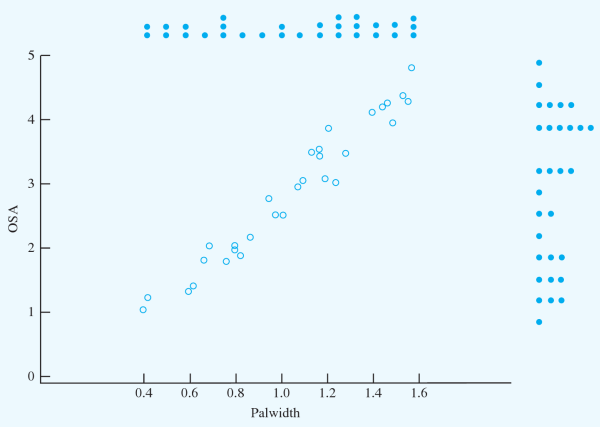
\includegraphics[width=4in]{NotesChap3_1.jpg} 
	   \caption{Example of a scatterplot}
	   \label{fig:example_scatterplot}
	\end{figure}
	
	\subsection{Correlation} %%% Section 3.2
	In order to make precise statements and draw reliable conclusions from the data, we must 
	go beyond pictures and find \textbf{Correlation Coefficient} which is a quantitative 
	assessment of the strength of relationship between $x$ and $y$ values in a set of pairs. \\
	
	A \textit{positive} relationship is one where both $x$ and $y$ tend to increase together. A 
	\textit{negative} relationship is one where $y$ tends to decrease as $x$ increases. A 
	strong positive or negative relationship can be linear or curved in appearance so long as x 
	and y tend to be clustered together in particular pattern.
		
	\p{Pearson's sample correlation}
		This sample correlation is $r$ given by the following equation:
		\[ r = \frac{\sum(x_i-\bar{x})(y_i-\bar{y})}{\sqrt{\sum(x_i-\bar{x})^2}\sqrt{\sum(y_i-\bar{y})^2}}  
		\]
		\[ = \frac{S_{xy}}{\sqrt{S_{xx}}\sqrt{S_{yy}}} \]
		Computing formulas for the three summation quantities are:
		\[ S_{xx} = \sum x_i^2-\frac{\left(\sum x_i\right)^2}{n} \]
		\[ S_{yy} = \sum y_i^2-\frac{\left(\sum y_i\right)^2}{n} \]
		\[ S_{xy} = \sum x_iy_i-\frac{\left(\sum x_i\right)\left(\sum y_i\right)}{n} \]
		
	\p{Properties of r}
		\begin{itemize}
			\item{The value of r does not depend on the unit of measurement for either variable, 
			meaning the correlation coefficient measures the inherent strength of relationship 
			between two numerical variables.}
		
			\item{The value of r does not depend on which of the two variables is labeled x.}
		
			\item{The value of r is between -1 and +1. A value near the upper limit is indicative of 
			a substantial positive relationship, whereas an r close to the lower limit suggests a 
			prominent negative relationship. }
		
			\item{r = 1 only when all the points in a scatterplot of the data lie exactly on a straight 
			line that slopes upward. Similarly, r = -1 only when all the points lie exactly on a 
			downward sloping line.}
		
			\item{The value of r is a measure of the extent to which x and y are \textbf{linearly} 
			related. The extent to which the points in the scatterplot fall close to a straight line.}
		\end{itemize}
		
	\p{The Population Correlation Coefficient}
		Pearson's r measures how strongly the x and y values in a \textit{sample} of pairs are 
		related to one another. There is an analogous measure of how strongly x and y are related 
		in the entire population of pairs from which the sample was obtained. This is called the 
		\textbf{population correlation coefficient} and is denoted by $\rho$. $\rho$ satisfies 
		properties paralleling those of r:
		\begin{itemize}
			\item{$\rho$ is a number between -1 and +1 that does not depend on the unit of 
			measurement for either x or y, or on which variable is labeled x and which is labeled 
			y}.
			\item{$\rho$ = +1 or -1 if and only if all pairs in the population lie exactly on a straight 
			line.}
		\end{itemize}
		
	\p{Correlation and Causation}
		Be sure to remember that just because a value of r is close to 1 does not mean that 
		relatively large values of one variable \textit{cause} relatively large values of the other 
		variable.
	
	\subsection{Fitting a Line to Bivariate Data} %%% Section 3.3
	Given two numerical values of x and y, the general objective of \textit{regression analysis} i
	s to use the information about x to draw some type of conclusion concerning y. The 
	different roles played by the two variables are reflected in standard terminology: y is called 
	the \textbf{dependent} or \textbf{response variable}, and x is referred to as the 
	\textbf{independent, predictor, or explanatory variable}. 
		
	A scatterplot of y vs x frequently exhibits a linear pattern. In such cases, it is natural to 
	summarize the relationship between the variables by finding a line that is as close as 
	possible to the points in the plot.
		
	\p{Fitting a Straight Line} Often when making a scatterplot, you can place a line 
		that generally summarizes the scatterplot and then each point will have a deviation from 
		that line. In order to find the best fitting line, we need to find the \textbf{Least Squares 
		Line}. To find that we have to minimize the following sum:
		\[ \sum[y_i-(a+bx_i)]^2 = [y_1-(a+bx_1)]^2+...+[y_n-(a+bx_n)]^2 \]
		To find this equation, let $g(\tilde{a},\tilde{b}) = \sum[y_i - (\tilde{a}+
		\tilde{b}x_i)]^2$. Then the intercept a and the slope b of the least squares line are the 
		values of $\tilde{a}$ and $\tilde{b}$ that minimize $g(\tilde{a},\tilde{b})$. 
		These minimizing values are obtained by taking the partial derivative of the g function first 
		with respect to $\tilde{a}$ and then with respect to $\tilde{b}$, and equating these 
		two partial derivatives to zero. \\
		
		The slope b of the least squares line is given by
		\[ b = \frac{\sum x_iy_i - \left(\sum x_i\right)\left(\sum y_i\right) / n}{\sum x_i^2 - \left(\sum 
		x_i\right)^2 / n} = \frac{S_{xy}}{S_{xx}} \]
		The vertical intercept a of the least squares line is given by
		\[ a = \bar{y} - b\bar{x} \]
		The equation of the least squares line is often written as $\hat{y} = a + bx$, where the hat 
		above the y emphasizes that $\hat{y}$ is a prediction of y that results from the substitution 
		of any particular x value into the equation.
		
		The least squares line should not be used to make a prediction for an x value much 
		beyond the range of the data. The danger of extrapolation is that the fitted relationship 
		may not be valid for such x values.
		
	\p{Regression}
		The term comes from the relationship between the least squares line and the sample 
		correlation coefficient. A little Algebraic manipulation yields:
		\[ b = r\left(\frac{s_y}{s_x}\right) \text{} \hat{y} = \bar{y} + r\left(\frac{s_y}{s_x}\right)(x-
		\bar{x} \]
		When $-1 < r < 1$, for \textit{any} $x$ value, the corresponding predicted value $\hat{y}$ 
		will be closer in terms of standard deviations to $\bar{y}$ than is $x$ to $\bar{x}$; that is, $
		\hat{y}$ is pulled toward (regressed toward) the mean $y$ value. This \textbf{regression 
		effect} was first noticed by Sir Francis Galton in the late 1800s when he studied the 
		relation between father's height and son's height; The predicted height of a son was 
		always closer to the mean height than was his father's height. 
		
	\p{Assessing the Fit of the Least Squares Line}
		How much of the observed variation in $y$ can be attributed to the approximate linear 
		relationship and the fact that $x$ is varying? A quantitative assessment is based on the 
		vertical deviations from the least squares line. 
		
		Variation in $y$ can be effectively be explained by an approximate straight-line 
		relationship when the points in the scatterplot fall close to the least squares line -- that is, 
		when the residuals are small in magnitude. A natural measure of variation about the least 
		squared line is the sum of the squared residuals.
		
		\textbf{Residual sum of squares}, denoted by \textbf{SSResid}, is given by:
		\[ \text{SSResid} = \sum(y_i-\hat{y})^2 = (y_1-\hat{y}_1)^2 +...+ (y_n-\hat{y}_n)^2 \]
		(Alternatively called \textit{error sum of squares} and denoted by SSE).\\
		\textbf{Total sum of squares}, denoted by \textbf{SSTo}, is defined as
		\[ \text{SSTo} = \sum(y_i-\bar{y})^2 \]
		Alternatie notation for SSTo is $S_{yy}$, and a computing formula is
		\[ \sum y_i^2 - \frac{\left(\sum y_i\right)^2}{n} \]
		A computing formula for residual sum of squares makes it unnecessary to calculate the 
		residuals:
		\[ \text{SSResid} = \text{SSTo} - bS_{xy} \]
		because $b$ and $S_{xy}$ have the same sign, $bS_{xy}$ is a positive quantity unless 
		$b=0$, so the computing formula shows that SSResid = SSTo if $b=0$ and SSResid < 
		SSTo otherwise.
		
		SSResid is the amount of variation in $y$ that cannot be attributed to the linear 
		relationship between $x$ and $y$. \\
		
		The \textbf{coefficient of determination}, denoted by $r^2$, is given by
		\[ r^2 = 1- \frac{\text{SSResid}}{\text{SSTo}} \]
		It is the proportion of variation in the observed $y$ values that can be explained by a linear 
		relationship between $x$ and $y$ in the sample.
		
	\p{Standard Deviation About the Least Squares Line}
		The \textbf{standard deviation about the least squares line} is given by
		\[ s_e = \sqrt{\frac{\text{SSResid}}{n-2}} \]
		Roughly speaking, $s_e$ is the typical amount by which an observation deviates from the 
		least squares line.
		
	\p{Plotting the Residuals (Optional}
		A desirable plot exhibits no particular pattern, such as curvature or much greater spread in 
		one part of the plot than in another part. Looking at a residual plot after fitting a line 
		amounts to examining $y$ after removing any linear dependence on $x$. This can 
		sometimes more clearly show the existence of a nonlinear relationship. \\
		
		A point that is far off typically means that there is some unusual behavior such a recording 
		error, non-standard experimental condition or atypical experimental subject.	

	\subsection{Nonlinear Relationships} %%% Section 3.4
	A scatterplot of bivariate data frequently shows curvature rather than a linear pattern. In this 
	section, we discuss several different ways to fit a curve to such data.
	
	\p{Power Transformations}
		Suppose that the general pattern is curved and monotonic. In this case, it is often 
		possible to find a \textbf{power transformation} for $x$ and $y$ so that there is a linear 
		pattern in a scatterplot of the transformed data. By a power transformation, we mean the 
		use of exponents $p$ and $q$ such that the transformed values are $x\prime = x^p$ and/
		or $y\prime = y^q$; the relevant scatterplot is of the $(x\prime ,y\prime)$ pairs. \\
	
		\begin{center}
			Power Transformation ladder: \\
			Transformed value = $(original value)^{POWER}$
			\begin{tabular}{ c c c } \hline
				Power & Transformed value & Name \\ \hline
				3 & $(Original value)^3$ & Cube \\
				2 & $(Original value)^2$ & Square \\
				1 & Original value & No transformation \\
				$\frac{1}{2}$ & $\sqrt{Original value}$ & Square root \\
				$\frac{1}{3}$ & $\sqrt[3]{Original value}$ & Cube root \\
				0 & Log(original value) & Logarithm \\
				-1 & $\frac{1}{original value}$ & Reciprocal \\
			\end{tabular} \\
			
			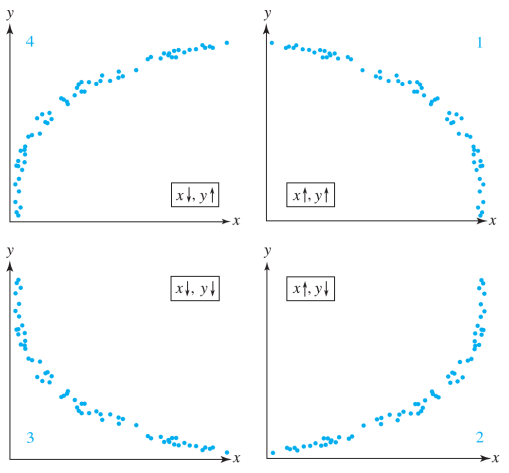
\includegraphics[width=2in]{transformation_guide.jpg}
		\end{center}
	
	\p{Fitting a Polynomial Function}
		Sometimes the general patter of curvature in a scatterplot is not monotonic. In such 
		instances, it is reasonable to fit a quadratic function $a + b_1x + b_2x^2$, whose graph is 
		a parabola, to the data. If the quadratic coefficient $b_2$ is positive, the parabola turns 
		upward, whereas it turns downward if $b_2$ is negative. Just as in fitting a straight line, 
		the principle of least squares can be employed to find the best-fit quadratic. The 
		\textbf{least squares coefficients $a, b_1, \text{and} b_2$} are the values of $\tilde{a}, 
		\tilde{b_1}, \text{and} \tilde{b_2}$ that minimize
		
		\[ g(\tilde{a},\tilde{b_1},\tilde{b_2}) = \sum_i [y_i-(\tilde{a}+\tilde{b_1}x_i+\tilde{b_2}
		x_i^2)]^2 \]
		
		Which is the sum of squared vertical deviations from the points in the scatterplot to the 
		parabola determined by the quadratic with coefficients $\tilde{a},\tilde{b_1},\tilde{b_2}$. 
		Taking the partial derivative of the $g$ function first with respect to $\tilde{a}$, then with 
		respect to $\tilde{b_1}$, and finally with respect to $\tilde{b_2}$, and equating these three 
		expressions to zero gives three equations in three unknowns. These \textit{normal 
		equations} are again linear in the unknowns, but because there are three rather than just 
		two, there is no explicit elementary expression for their solution. Instead, matrix algebra 
		must be used to solve the system numerically for each different data set. \\
		
		The methodology employed to fit a quadratic is easily extended to fit a higher-order 
		polynomial. For example, using the principle of least squares to fit a cubic equation gives 
		a system of normal equations consisting of four equations in four unknowns. The 
		arithmetic is best left to a statistical computer package. In practice, a cubic equation is 
		rarely fit to data, and iti s virtually never appropriate to fit anything of higher order than 
		this.
		
	\p{Smoothing a Scatterplot}
		Sometimes the pattern in a scatterplot is too complex for a line or curve of a particular 
		type (e.g., exponential or parabolic) to give a good fit. Statisticians have recently 
		developed some more flexible methods that permit a wide variety of patterns to be 
		modeled using the same fitting procedure. One such method is LOWESS, short for 
		\textit{locally weighted scatterplot smoother}. Let $(x\ast,y\ast)$ denote a particular one of 
		the $n$ $(x,y)$ pairs in the sample. The $\hat{y}$ value corresponding to $(x\ast,y\ast)$ 
		is obtained by fitting a straight line using only a specified percentage of the data (e.g, 
		25\%) whose $x$ values are closest to $x\ast$. Furthermore, rather than use "ordinary" 
		least squares, which gives equal weight to all points, those with $x$ values closer to $x
		\ast$ are more heavily weighted than those whose $x$ values are farther away. The 
		height of the resulting line above $x\ast$ is the fitted value $\hat{y}\ast$. This process is 
		repeated for each of the $n$ points, so $n$ different lines are fit (you surely wouldn't want 
		to do all this by hand). Finally, the fitted points are connected to produce a LOWESS 
		curve.
		
		\begin{center}
			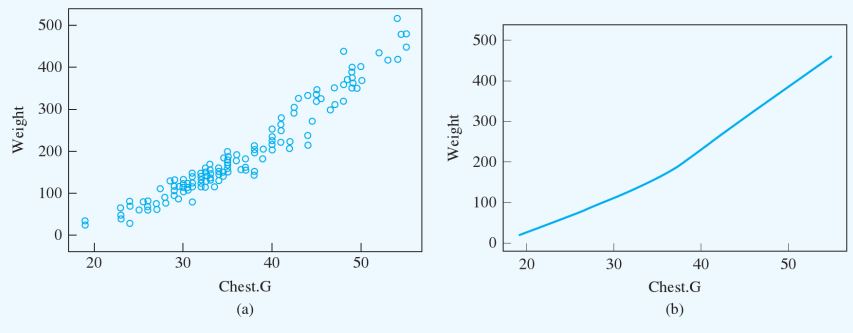
\includegraphics[width=4in]{lowess_example.jpg}
		\end{center}
	
	\subsection{using More Than One Predictor} %%% Section 3.5
	
	In many situations, predictions of $y$ values can be improved and more observed $y$ variation 
	can be explained by utilizing information in two or more explanatory variables. Notation is a bit 
	more complex than in the case of a single predictor. Let
	\begin{align}
		k &= \text{number of explanatory variables or predictors} \\
		n &= \text{sample size}
	\end{align}
	and $x_1,x_2,...,x_k$ denote the $k$ predictors, so that each observation will consist of $k+1$ 
	numbers: the value of $x_1$, the value of $x_2,...,$ the value of $x_k$, and the value of $y$. 
	Also let
	\[ x_{ij} = \text{value of the predictor $x_i$ in the $i$th observation} \]
	so
	\[ first observation = (x_{11},x_{21},...,x_{k1},y_1) \]
	\[ ... \]
	\[ \text{$n$th observation} = (x_{1n},x_{2n},...,x_{kn},y_n) \]
	
	\p{Example}
	\begin{center}
		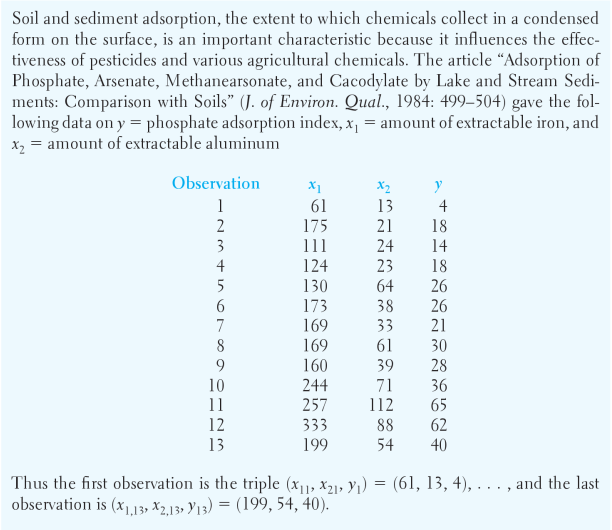
\includegraphics[width=4in]{example_315.jpg}
	\end{center}
	
	A scatterplot of this data would represent each observation as a point in a three-dimensional 
	coordinate system, which is obviously difficult to construct or visualize. Partial information about 
	the relationship between the variables can be obtained by forming a \textbf{scatterplot matrix}. 
	This is just a collection of two-dimensional scatterplots, arranged in a square array, in which 
	each variable is plotted against every other variable. Here is a scatterplot matrix of the data in 
	the previous example: 
	
	\begin{center}
		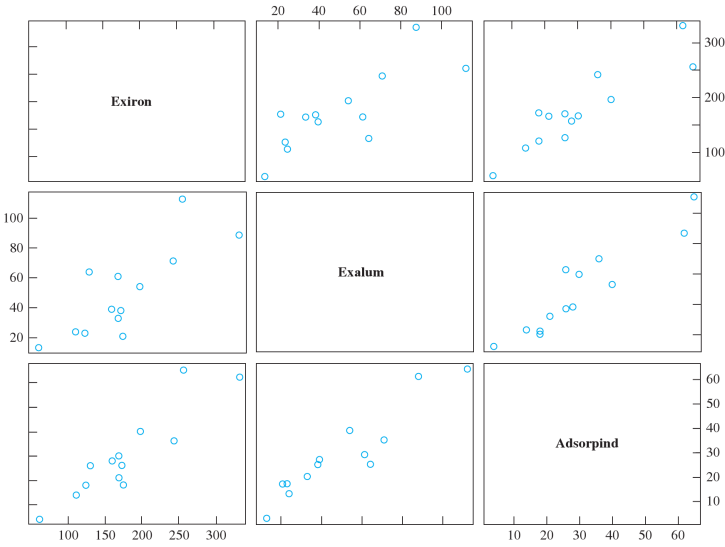
\includegraphics[width=4in]{ex_315_scatterplot_matrix.jpg}
	\end{center}
	
	\p{Fitting a Linear Function}
		We now consider fitting a relation of the form: 
		\[ y \approx a + b_1x_1 + b_2x_2 +...+ b_kx_k \]
		The reasonableness of this approximation depends on patterns in the scatterplot matrix 
		and other characteristics of the data to be considered shortly. As with bivariate data, the 
		values of $a, b_1,...,b_k$ should be selected to give the best fit. \\
		The \textbf{least squares coefficients $a,b_1,b_2,...,b_k$} are the values of $\tilde{a},
		\tilde{b_1},...,\tilde{b_k}$ that minimize
		\[ g(\tilde{a},\tilde{b_1},...,\tilde{b_k}) = \sum_{j-1}^n [y_j - (\tilde{a} + \tilde{b_1}x_{1j}+...+
		\tilde{b_k}x_{kj})]^2 \]
		The g() function is the sum of squared deviations between observed $y$ values and what 
		would be predicted by $\tilde{a} + \tilde{b_1}x_1 +...+ \tilde{b_k}x_k$.
		
	\subsection{Joint Distributions} %%% Section 3.6

\clearpage	 %%%%% I guess we skipped this chapter?
\section{Obtaining Data} %%% Chapter 4 Page 161

	\subsection{Operational Definitions} %%% Section 4.1
	
	\subsection{Data from Sampling} %%% Section 4.2
	
	\subsection{Data from Experiments} %%% Section 4.3
	
	\subsection{Measurement Systems} %%% Section 4.4

\clearpage	
\section{Probability and Sampling Distributions} %%% Chapter 5 Page 194

	\subsection{Chance Experiments} %%% Section 5.1
	A \textbf{chance experiment}, also called a \textbf{random experiment}, is simply an activity or 
	situation whose outcomes, to some degree, depend on chance. To decide whether a given 
	activity qualifies as a chance experiment, ask yourself the question, will I get exactly the same 
	result if I repeat the experiment more than once? If no, then the experiment is a chance 
	experiment.
	
	\p{Events} ~\\
	Underlying the computations of probability is an organized system for describing and working 
	with the outcomes of chance experiments. These outcomes can be divided into two types: 
	\textbf{simple events}, which are the individual outcomes of an experiment and, more generally, 
	\textbf{events}, which consist of collections of simple events. For instance, the chance 
	experiment of conducting a series of stress tests on three metal parts has eight possible 
	outcomes. Each of these eight outcomes is a simple event, which, taken together, form the 
	\textbf{sample space} of the experiment.
	
	\p{Depicting Events} ~\\
	Various devices have been created to help visually describe the events in a sample space. 
	\textbf{Tree diagrams} are especially useful for depicting experiments that are conducted in a 
	sequence of steps, such as our example of testing three metal parts. Beginning at the left, each 
	step in the sequence is given its own set of branches, which themselves form the starting points 
	for all branches to their right. The figure below shows a tree diagram example:
	
	\begin{figure}[!htbp]
	   \centering
	   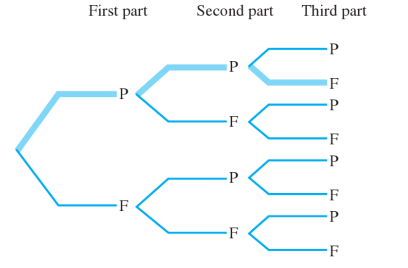
\includegraphics[width=4in]{figure5_2.jpg} 
	   \caption{Tree diagram for the experiment of selecting and testing three mechanical parts 
	   (branches forming the simple event PPF are shown shaded)}
	   \label{fig:figure5_2}
	\end{figure}
	
	Another visual device, the \textbf{Venn diagram}, is especially useful for depicting 
	\emph{relationships} between events. Venn diagrams are simple two-dimensional figures, often 
	rectangles or circles, whose enclosed regions are intended to depict a collection of simple 
	events, called \emph{points}, in a sample space.\\
	
	Venn diagrams and tree diagrams are indispensable tools in many parts of probability theory, but 
	they are not essential to conducting statistical studies.
	
	\p{Forming New Events} ~\\
	Simple events are fundamental to describing chance experiments, but the events that are of 
	most interest are usually much more complex. One of the primary methods for creating complex 
	events and, therefore, for unraveling them, involves the use of the words \emph{and, or}, and 
	\emph{not}. The following box shows how these words are used to build new events from old 
	ones.
	
	\p{Definitions} ~\\
	For a chance experiment and any two events A and B:
	\begin{enumerate}
		\item{The event \textbf{A or B} consists of all simple events that are contained in either A or 
		B. \textbf{A or B} can also be described as the event that \emph{at least one} of A or B 
		occurs.}
		\item{The event \textbf{A and B} consists of all simple events common to both A and B. 
		\textbf{A and B} can be described as the event that \emph{both} A and B occur.}
		\item{The event \textbf{$A^'$}, called the \textbf{complement of A, consists of all simple 
		events that are \emph{not} contained in A. \textbf{$A^'$} is the event that A does not occur.}
	\end{enumerate}
	For example:
	\begin{center}
		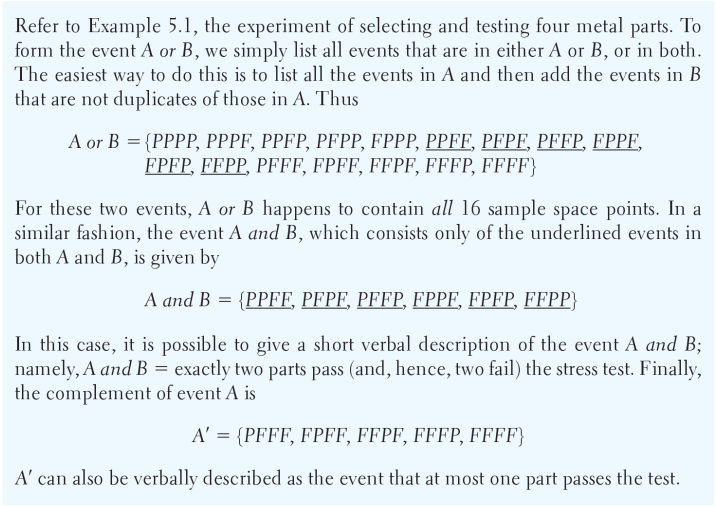
\includegraphics[widht=4in]{example5_3.jpg}
	\end{center}
	
	When two events A and B have no simple events in common, we say that they are 
	\textbf{mutually exclusive \text{or} disjoint}. More intuitively, mutually exclusive events are ones 
	that cannot occur simultaneously.

	\subsection{Probability Concepts} %%% Section 5.2
	
	\subsection{Conditional Probability and Independence} %%% Section 5.3
	
	\subsection{Random Variables} %%% Section 5.4
	
	\subsection{Sampling Distributions} %%% Section 5.5
	
	\subsection{Describing Sampling Distributions} %%% Section 5.6
	Just as histograms of sample data provide approximations to population distributions, sampling experiments (Section 5.5) furnish approximate pictures of sampling distributions. We now turn our attention to developing more precise summaries of sampling distributions. In this section, we study in some detail the ex

\clearpage	 %%%%%% Looks like we're skippin this chapter too?
\section{Quality and Reliability} %%% Chapter 6 Page 246

	\subsection{Terminology} %%% Section 6.1
	
	\subsection{How Control Charts Work} %%% Section 6.2
	
	\subsection{Control Charts for Mean and Variation} %%% Section 6.3
	
	\subsection{Process Capability Analysis} %%% Section 6.4
	
	\subsection{Control Charts for Attributes Data} %%% Section 6.5
	
	\subsection{Reliability} %%% Section 6.5

\clearpage	
\section{Estimation and Statistical Intervals} %%% Chapter 7 Page 293

The general objective of a statistical inference is to use sample information as a basis for drawing various types of conclusions. In an estimation problem, we want to make an educated guess about the value of some population characteristic or parameter, such as the population mean battery lifetime $\mu$, the proportion $\pi$ of all components of a certain type that need service while under warranty, or the difference $\mu_1-\mu_2$ between the population mean lifetimes for two different types of batteries. The simplest type of estimate is a \emph{point estimate}, a single number that represents our best guess for the value of the parameter.

	\subsection{Point Estimation} %%% Section 7.1
	A \textbf{point estimate} of some parameter $\theta$ is a single number, calculated from sample 
	data, that can be regarded as an educated guess for the value of $\theta$. \\
	A point estimate is usually obtained by selecting a suitable statistic and calculating its value for 
	the given sample data. For example, a natural statistic to use for estimating a population mean $
	\mu$ is the sample mean $\bar{x}$, and a sensible way to estimate a population variance $
	\sigma^2$ is to compute the value of the sample variance $s^2$. The statistic used to calculate 
	an estimate is sometimes called an \textbf{estimator}, and the symbol $\hat{\theta}$ is frequently 
	used to denote either the estimator or the resulting estimate. Thus the statement
	\[ \hat{\mu} = \bar{x} = 32.5 \]
	says that the point estimate of the population mean $\mu$ is 32.5 and that this estimate was 
	calculated using the sample mean $\bar{x}$ as the estimator.
	
	\begin{figure}[!htbp]
	   \centering
	   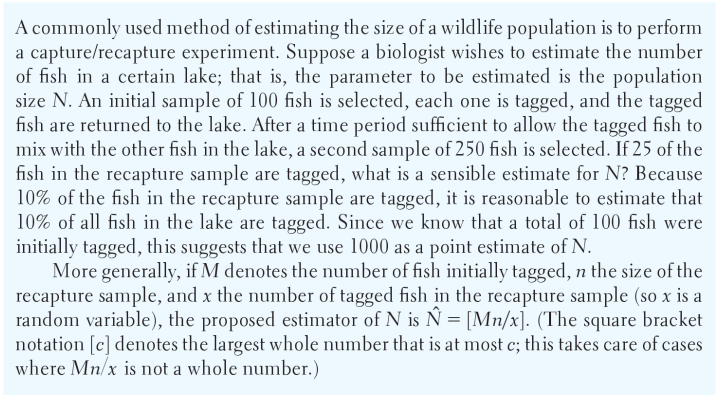
\includegraphics[width=4in]{example7_1.jpg} 
	   \caption{Example 7.1}
	   \label{fig:example7_1}
	\end{figure}
	
	Frequently, there is more than one estimator that can sensibly be used to calculate an estimate, 
	as the following example shows.
	
	\begin{figure}[!htbp]
	   \centering
	   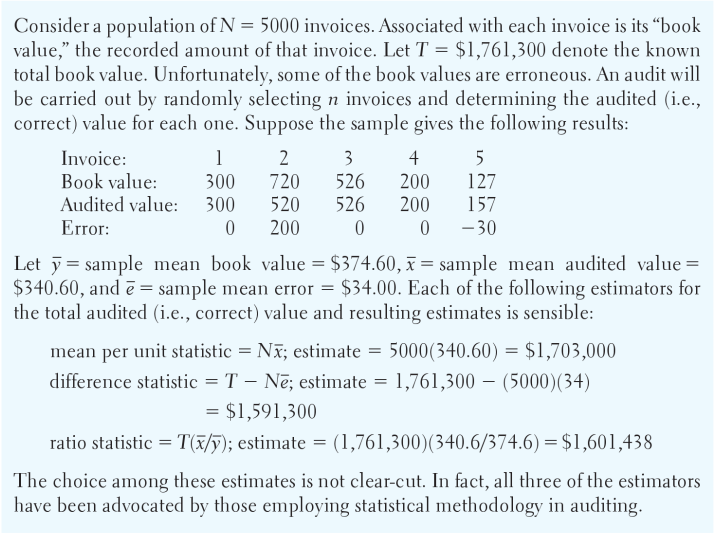
\includegraphics[width=4in]{example7_2.jpg} 
	   \caption{Example 7.2}
	   \label{fig:example7_2}
	\end{figure}
	
	\p{Properties of Estimators} One desirable property that a good estimator should possess is that 
	it be \textbf{unbiased}. An estimator is unbiased if, in repeated random samples, the numerical 
	values of the estimator stack up around the population parameter that we are trying to estimate. 
	An often used analogy is to think of each value of an estimator as a shot fired at a target, the 
	target being the population parameter of interest. As long as all the shots fall in a pattern with the 
	target value in the \emph{middle}, we say that the shots are unbiased. Notice that we do not 
	require that any of the individual shots actually hit the target; we require only that they be 
	centered around the target value. If the majority of the shots are centered somewhere else, then 
	we say that they exhibit a certain amount of \textbf{bias}.
	
	\p{Definition} ~ \\
	Denote a population parameter generically by the letter $\theta$ and denote any estimator of 
	this parameter by $\hat{\theta}$. Then $\hat{\theta}$ is an \textbf{unbiased} estimator if $
	\mu_{\hat{\theta}} = \theta$. Otherwise, $\hat{\theta}$ is said to be biased, and the quantity $
	\mu_{\hat{\theta}} - \theta$ is called the \textbf{bias} of $\hat{\theta}$. \\
	
	Unbiasedness does not imply that the estimate computed from any particular sample will 
	coincide with the value of the parameter being estimated. Consider, for example, using the 
	sample proportion $p$ to estimate the population proportion $\pi$ based on a sample of size 
	$n=25$, and suppose that $\pi = 0.7$. Then $\mu_p=0.7$, so the sampling distribution of $p$ is 
	centered at 0.7. However, with $x$ denoting the number of "successes" in the sample, $p = 
	\frac{x}{25} \not= 0.77$ for any possible value of $x$. That is, even though $p$ is unbiased for 
	estimating $\pi$, the value of the estimate calculated from any particular sample will inevitably 
	differ from $\pi$. \\
	
	A second desirable property that estimators often possess is consistency. If $\hat{\theta}$ 
	denotes an estimator of some population parameter $\theta$, then $\hat{\theta}$ is said to be 
	\textbf{consistent} if the probability that it lies close to $\theta$ increases to 1 as the sample size 
	increases. That is, as you increase $n$, it becomes more and more likely that such estimators 
	will be very close to the parameter they are intended to estimate. The most common method for 
	showing that an estimator is consistent is to show that its standard error decreases as the 
	sample size increases.
	
	\p{Definition} ~\\
	If the probability that an estimator $\hat{\theta}$ falls close to a population parameter $\theta$ 
	can be made as near to 1 as desired by increasing the sample size $n$, then $\hat{\theta}$ is 
	said to be a \textbf{consistent} estimator of $\theta$.
	
	\subsection{Large-Sample Confidence Intervals for a Population Mean} %%% Section 7.2
	
	\subsection{More Large-Sample Confidence Intervals} %%% Section 7.3
	
	\subsection{Small-Sample Intervals Based on a Norm. Pop. Distr.} %%% Section 7.4
	
	\subsection{Intervals for $\mu_1 - \mu_2$ based on Norm. Pop. Distr.} %%% Section 7.5
	
	\subsection{Other Topics in Estimation (Optional)} %%% Section 7.6

\clearpage	
\section{Testing Statistical Hypotheses} %%% Chapter 8 Page 352

	\subsection{Hypotheses and Test Procedures} %%% Section 8.1
	
	\subsection{Tests Concerning Hypotheses About Means} %%% Section 8.2
	
	\subsection{Tests Concerning Hypotheses About a Categorical Population} %%% Section 8.3
	
	\subsection{Testing the Form of a Distribution} %%% Section 8.4
	
	\subsection{Further Aspects of Hypothesis Testing} %%% Section 8.5

\clearpage	
\section{The Analysis of Variance} %%% Chapter 9 Page 413

	\subsection{Terminology and Concepts} %%% Section 9.1
	
	\subsection{Single-Factor ANOVA} %%% Section 9.2
	
	\subsection{Interpreting ANOVA Results} %%% Section 9.3
	
	\subsection{Randomized Block Experiments} %%% Section 9.4

\clearpage	
\section{Experimental Design} %%% Chapter 10 Page 445

	\subsection{Terminology and Concepts} %%% Section 10.1
	
	\subsection{Two-Factor Designs} %%% Section 10.2
	
	\subsection{Multifactor Designs} %%% Section 10.3
	
	\subsection{$2^k$ Designs} %%% Section 10.4
	
	\subsection{Fractional Factorial Designs} %%% Section 10.5

\clearpage	
\section{Inferential Methods in Regression and Correlation} %%% Chapter 11 Page 503

	\subsection{Regression Models Involving a Single Independent Variable} %%% Section 11.1
	
	\subsection{Inferences About the Slope Coefficient} %%% Section 11.2
	
	\subsection{Inferences Based on the Estimated Regression Line} %%% Section 11.3
	
	\subsection{Multiple Regression Models} %%% Section 11.4
	
	\subsection{Inferences in Multiple Regression} %%% Section 11.5
	
	\subsection{Further Aspects of Regression Analysis} %%% Section 11.6
	
\clearpage
\section{Appendix Tables} %%% Appendix tables Page 581









%%%%%%%%%%%%%%%%%%%%%%%%%%%%%%%%%%%%%%%%%%%%%%%%%%%%%%%%%%%%%%%%%%%%%OTHER NOTES%%%%%%%%%%%%%%%%%%%%%%%
%%%%%%%%%%%%%%%%%%%%%%%%%%%%%%%%%%%%%%%%%%%%%%%%%%
\iffalse
\section{Day 1: Intro to Stats 3/31/2015}
	
	\p{Definition}
	the practice or science of collecting and analyzing numerical data in large quantities, especially
	for the purpose of inferring proportions in a whole from those in a representative sample.
	
	\subsection{Variables}
	Variables: any characteristic whose value may change form one object to another in the population.
	\subsection{Types}
		\subsubsection{Categorical}
			\p{Nominal Scale}
			 No ordering of the possible values. Ex: any type of binary or yes/no question are
			 nominal. Things like blood type as well.
			 
			 \p{Ordinal Scale}
			 Natural ordering of the possible values. The difference or mean of values is not
			 defined. Ex: S/M/L shirts and hat sizes, Likert scale responses (strongly disagree
			 to Strongly agree).

		\subsubsection{Quantitative}
		The Average in a Quantitative variable needs to make sense in order to be quantitative.
			\p{Continuous}
			Any value in an interval of real numbers is possible.
			
			\p{Discrete}
			All possible values can be listed (Countable).
			
			\p{Interval Scale}
			A numeric value variable for which differences make sense but there is no natural
			zero. Ex: degrees fahrenheit, degrees celsius arbitrary zero.
			
			\p{Ratio Scale}
			A numeric variable for which differences and ratios make sense. i.e. there is an
			absolute zero. Ex: Snow pack, rainfall.
			
	\subsection{Descriptive Stats}
	Goal is to describe and summarize data numerically or graphically. There are several
	different methods to do this:
		
		\subsubsection{Quantitative}
			\p{Stem and leaf plot}
			\p{Dot plot}
			\p{Frequency table}
			\p{Histogram}
			Distribution of data. The smooth curve drawn on a histogram is called a 
			\textbf{Density Curve} and is a theoretical distribution of a variable.
			
		\subsubsection{Categorical}
			\p{Frequency table}
			\p{Bar chart}

\section{Day 2:  4/2/2015}

	\subsection{Distribution of a Variable}
	\p{Definition}
	The distribution of a variable refers to the values a variable can take on and how frequently it
	takes on those values.
	
	We attach adjectives that refer to the shape of a distribution when viewing a histogram.
	
		%Include image of different distributions:
		\subsubsection{Types of distributions}
		
			Properties of Unimodal graphs: Symmetry.

			\p{Normal / Bell Curve / Gaussian} asdf
			\begin{figure}[!htb]
				\centering
				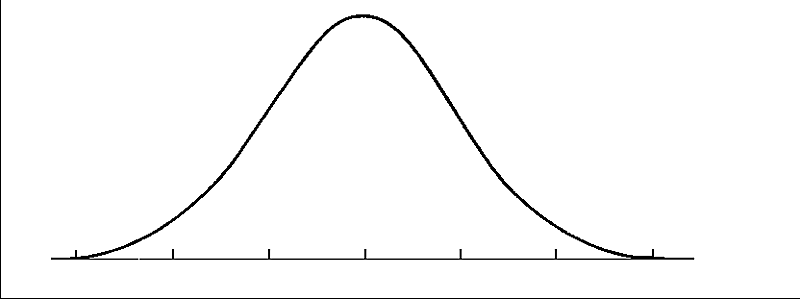
\includegraphics[width=0.75\textwidth]{BellDistribution.png}
				\caption{Example of a Bell Curve}
			\end{figure} 
			Examples: heights, SAT scores
			\p{Uniform}
			\begin{figure}[!htb]
				\centering
				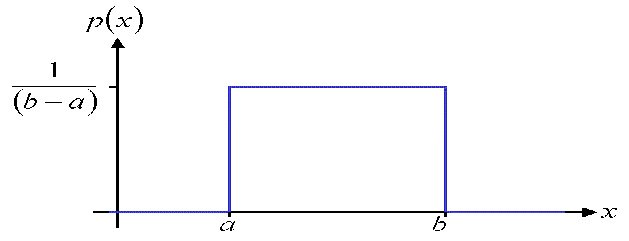
\includegraphics{UniformDistribution.png}
				\caption{Example of a Uniform Distribution}
			\end{figure} 
			Example: Odds of a dice roll
			\p{Positively or right skewed}
			\begin{figure}[!htb]
				\centering
				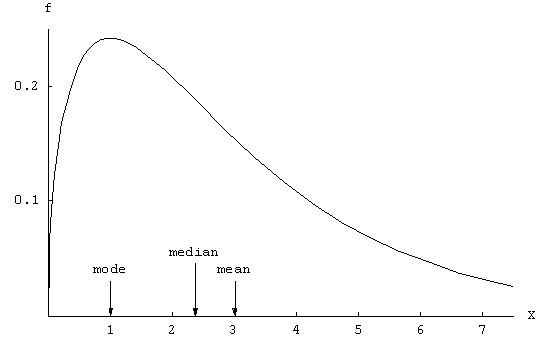
\includegraphics{RightSkewed.png}
				\caption{Example of a Right or Positive Skewed Distribution}
			\end{figure}
			Example: Number of pets, hours of television per week
			\p{negatively or left skewed}
			\begin{figure}[!htb]
				\centering
				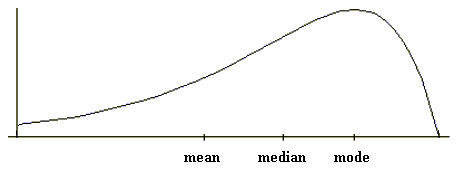
\includegraphics{LeftSkewed.png}
				\caption{Example of a Left or Negative Skewed Distribution}
			\end{figure}
			\p{bimodal (two peaks)}
			When you say the mode of a distribution graph you refer to the peaks.
			Can occur if you're sampling 2 different populations.
			\begin{figure}[!htb]
				\centering
				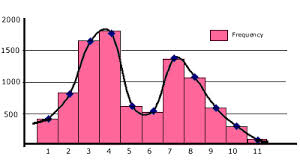
\includegraphics{Bimodal.png}
				\caption{Example of a Bimodal Distribution}
			\end{figure}
		
		\subsubsection{Continuous Distribution (Density)}
		The smooth curve drawn on a histogram is called a **Density Curve** and is a theoretical
		distribution of a variable. For a continuous distribution of some variable x, model the
		density curve by f(x) or the **Density Function** P(x). with domain D in (-infinity, infinity) = Real numbers.
		P(x) must satisfy:
		\begin{itemize}
			\item{f(x) >= 0 for all x in D}
			\item{integral of f(x) in D with respect to x equals 1}
			\item{For any a,b in D where (a < b) the proportion of values between a and b is (the integral from a to b of f(x) with respect to x) = P(a <= x <= b) (The probability that x is between a and b).}
		\end{itemize}
		If you have a continuous distribution, the probability that you will land on any specific point is always zero (P(x = a) = 0).
		
		\subsubsection{Discrete Distribution}
		For a discrete distribution of a variable $x$, model the probabilities of getting particular 
		values by a \textbf{probability mass function} $p(x)$. Domain $D$ is typically 
		$\{0, 1, 2, 3...\}$.
		$p(x)$ must satisfy:
		\begin{itemize}
			\item{$p(x) \ge 0$ for all $x$ in $D$}
			\item{$\sum_{k = 0}^{\infty} p(k) = 1$ (probability always between 0 ad 1)}
		\end{itemize}
	
		 $P(a \le x \le b) = \sum_{k = a}^{b} p(k)$ \\
		 $P(a < x < b) = \sum_{k = a + 1}^{b - 1} p(k)$. \\
		
		 $\int_{a}^{b} x^2 dx$
		
		\p{Examples} Some examples\\
		
		 Example 1: $f(x) = cx^8(1-x)$ \\
		Domain: $[0,1]$ \\
		$f$ is a density function. \\
		find $c$. \\
		
		 $\int_{0}^{1} x^8(1 - x) dx = \frac{1}{c}$ \\
		 $\int_{0}^{1} x^8 dx - \int_{0}^{1} x^9 dx = \frac{1}{c}$ \\
		 $\frac{x^9}{9} - \frac{x^{10}}{10} = \frac{1}{c}$ \\
		 $\frac{1}{9} - \frac{1}{10} = \frac{1}{c}$ \\
		 $c = 90$\\
		
		 Example 2: $f(x) = \frac{c}{1+x^2}$ \\
		$D = (-\infty, \infty)$
		find $c$. \\
		
		 $\int \frac{1}{1 + x^2} dx = arctan(x)$ \\
		 $c\int_{-\infty}^{\infty} f(x) dx = c [\lim_{x\to\infty} arctan(x) - \lim_{x\to -\infty} 
		arctan(x)]$ \\
		 $= c[\frac{\pi}{2} - (-\frac{\pi}{2})$ \\
		 $ = c\pi = 1$ \\
		 $ c = \frac{1}{\pi}$ \\
		
		 Example 3: what is $D = \{1, 2, ..., 20\}$ and what is $p(x)$ if we have a fair 20-sided die? \\
		
		 $p(1) = p(2) = ... = p(20) = \frac{1}{20}$ 
		
		\subsubsection{Important Distributions}
		
		\p{Normal Distribution}
		In the domain $D = (-\infty, \infty)$ 
		\[
			f(x) = \frac{1}{\sqrt{2\pi}\sigma} e^{\frac{-(x-\mu)^2}{2\sigma^2}}
		\]
		 The center is $\mu$ "mu" which is the mean (mode, average). \\
		 The shape is defined by $\sigma$ "sigma" which is the standard deviation.\\
		
		 A normal distribution is symmetric about $x = \mu$.
		
		\begin{figure}[!htb]
			\centering
			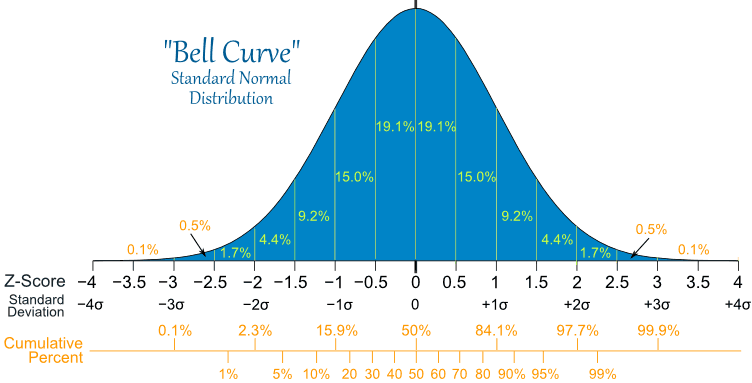
\includegraphics{StandardNormalDistribution.png}
			\caption{A Standard Normal Distribution}
		\end{figure}
		
		\p{Standard Normal Distribution}
		A standard normal distribution is a normal distribution but with $\mu = 0$ and $\sigma = 1$. In this case, the standard normal equation is $f(x) = \frac{1}{\sqrt{2\pi}} e^{\frac{-2^2}{2}}$.
		
		\p{Notation} notation \\
		 $X ~ N(\mu, \sigma) =$ "X follows a normal distribution with mean $\mu$ and standard deviation $\sigma$". $~ =$ "is distributed as". \\
		
		 $z is$ \\
		
\section{Day 3 4/7/15:}
		
		\p{Exponential family} Density is of form
		\[
			f(x) = \left\{
			\begin{array}{lr}
				\lambda e^{\lambda x} x > 0 \\
				0 & otherwise
			\end{array}
			\right.
		\]
		Parameters: $\lambda$ - Average number of events in one unit. \\
		                                      - Waiting time for a rare event. \\
		Example: time until next phone call or distance to next knot in plank of wood. //
		
		\p{Poisson Distribution}
		Has a mass function:
		\[
			p(k) = \frac{e^\lambda \lambda^k}{k!}
		\]
		$k = 0, 1, 2,....$ \\
		$\lambda$ average number of events in one unit \\
		\hspace{17pt} number of knots in 1 meter of wood\\
		$\lambda$ is the mean of the poisson distribution.
		\[
			mean = \sum_{k=0}^{\infty} kp(k) = \lambda
		\]
		
		From TMATH 126:
		\[
			e^x = \sum_{n=0}^{\infty} \frac{x^n}{n!}
		\]
		
		From TMATH 124: L'hoptal's rule:
		\[
			\lim_{x\to a} \frac{f(x)}{g(x)} = \lim_{x\to a} \frac{f\prime(x)}{g\prime(x)}
		\]
		Provided that the limits both go to the same thing. \\
		
		Another cheat sheet thing: if g is continuous
		\[
			\lim_{x\to a} g(f(x)) = g(\lim_{x\to a} f(x))
		\]
		
		From TMATH 124:
		\[
			e^x = \lim_{n\to\infty} (1 + \frac{x}{n})^n
		\]
		
		Now that we are all done with previous shit: Go to binomial distribution section.
		
		\p{Geometric Distribution}
		Example: Count number of count flips until you get heads ($H$) \\
		Let $\pi =$ probability of getting $H$, so $1-\pi =$ probability of $T$. Mass function:
		\[
			p(k) = (1-\pi)^{k-1}\pi
		\]
		
		Example 2: unfair coin: $\pi = \frac{1}{4}, $p(k=3) = (1-\frac{1}{4})^2\frac{1}{4} = \frac{9}
		{64}. 
		
		\p{Binomial Distribution}
		$\pi$ = probability of getting H \\
		Number of H I get if I flip a coin $n$ times. Mass function:
		\[
			p(k) = \left( \frac{n!}{(n-k)! k!} \pi^k (1-\pi)^{n-k} \right), k = 0,1,2,... (is number of heads)
		\]
		Example: Hoe many ways can I select a sample size of 2 from a class of 30? 435 How'd we get the answer? We did 30 choose 2
		
		Putting it all together! \\
		$X ~ Binomial(n, \pi)$ \\
		Assume that $n$ is big $(n \to \infty)$\\
		and $\pi$ is small $(\pi \to 0)$ \\
		Fix $\lambda > 0$, set $\pi = \frac{\lambda}{n}$ So if n goes to infinity then pi 
		goes to zero. \\
		
		Chance of getting k heads in in trials: \\
		\[
			\lim_{n\to\infty} (nchoosek) \left( \frac{\lamda}{n} \right)^k \left(1 - \frac{\lamda}{n}\right)^{n-k}
		\]
		\[
			\frac{n ... \left(n - k + 1\right)}{k!} \frac{\lambda^k}{n^k} \frac{\left(1 - \frac{\lamda}{n}\right)^n}{\left(1 - \frac{\lamda}{n}\right)^k}
		\]
		\[
			= \frac{\lambda^k}{k!} \lim_{n\to\infty} \frac{n(n-1)...(n-k+1)}{n^k} \frac{1}{(1-\frac{\lamda}{n})^k \frac{(1-\frac{\lamda}{n})^n}{1}
		\]
		\[
			= \frac{\lamda^k}{k!} e^{-\lamda}
		\]
		This is the mass function for poisson.
		
		% Put in what was written down on other paper
		
	\subsection{Chapter 2 Numerical studies}
	
		\subsubsection{For Data (histograms)}
		\p{Measures of Center} def: \\
		Sample mean = $\bar(x) = \frac{1}{n} \sum_{i = 1}^{n} x_i$ \\
		Sample median = $\tilde(x) = the middle observation$
		\[
			\tidle(x) = \left\{
				\begin{array}{l}
					The middle #, \lceil\frac{n}{2}\rceil # \\
					Average the middle two numbers
				\end{array}
			\right.
		\]
		
		$\tilde(x)$ is resistant to extreme observations \\
		$\bar(x)$ is not resistant to extreme observations \\
		
		\p{Measures of Variability or Spread} def:\\
		Sample Range = (maxvalue)-(minvalue) \\
		Sample Variance = $s_x^2 = \frac{1}{n-1} \sum_{i=1}^{n} (x_i - \bar(x))^2$ \\
		You get "n-1" differences from "n" observations \\
		You lose a degree of freedom when you find $\bar(x)$ \\
		Squaring works nicely in calculus \\
		if x,y independent: $s_{x+y}^2 = s_x^2 + s_y^2$.\\
		
		Sample standard deviation: 
		\[
			s_x = \sqrt{\frac{1}{n-1} \sum_{i=1}^{n} (x_i - \bar(x))^2}
		\]
		Same units as "x"\\
		
		Never calculate variance using defining formula. If you have to do it by hand: \\
		Computational formula:
		\[
			s_x^2 = \frac{1}{n-1} \left( \sum_{i = 1}{n} x_i^2 - \frac{1}{n} \left( \sum{i=0}{n} x_i \right)^2\right)
		\]
		
		\p{Other Measures} def:\\
		\textbf{Inter Quartile Range} is the difference between the first and third quartiles. It is the spread of the middle 50\% of the data and is resistant to extreme observations. \\
		
		Sample quartiles:
		\begin{itemize}
			\item{$Q_0$ = minimum
			\item{$Q_1$ = first quartile. 25\% below and 75\% above.}
			\item{$Q_2$ = second quartile. 50 below and above. median or $\tilde(x)$}
			\item{$Q_3$ = third quartile. 75 below 25 above}
			\item{$Q_4$ = maximum.
		\end{itemize}
		$Q_1$ is the median of the lower half of the data and $Q_3$ is the median of the upper half of the data. $Q_1$ and $Q_3$ are the only ones we actually call quartiles.
		
		
\section{Day 4 4/9/15:}

		\p{Box Plot} A Graphical representation of 5-number summary. In order to find the 5 number summary, you need to sort your data.
		
		%Include examples of box plots we did in class.
		
		\p{General notes:} Histograms are for data
		
		\subsection{2.1 Measures of center}
		Expected value of $X = E[X] = \mu_X$
		\[
			E[X] = \left\{
			\begin{array}{lr}
				\sum_{k}^{} kp(k) & discrete
				\int_{-\infty}^{\infty} xf(x)dx & continuous
			\end{array}
			\right.
		\]
		
		\p{Example} 6 sided fair die\\
		\[
			E(X) = \frac{1}{6} + 2 * \frac{1}{6} ...
		\]
		\[
			= \frac{\sum_{k=1}^{6} k}{6} = \frac{21}{6} = 3.5
		\]
		
		\p{Properties} of E \\
		If "c" is a constant (not random), $E[c] = c$. \\
		$E$ is a "linear operator": $E[aX + bY] = aE[X] + bE[Y]$.
		
		\subsection{2.2 Spread (variation)}
		Variance of $X$:
		\[
			V[X] = \left\{
			\begin{array}{lr}
				\sum_{k}^{} (k - E[X])^2 * p(k) & discrete
				\int_{-\infty}^{\infty} (x-E[X])^2 * f(x) dx & continuous
			\end{array}
			\right.
		\]
		
		$V[X]$ is an expected value of a function of $X$
		\[
			E[(X - E(X))^2]
		\end{display math}
		\[
			V[X] = E[X^2-2XE[X] + (E[X])^2]
		\]
		\[
			V[X] = E[X^2] - (E[X])^2
		\]
		
		\p{Properties} of V\\
		\[
			V[aX] = a^2V[X]
		\]
		
		if $X$ and $Y$ are independent, then $E[XY] = E[X]E[Y] and V[X+Y] = V[X] + V[Y]$ \\
		\textbf{Independence:} $X$'s and $Y$'s outcomes don't influence each other. \\
		\[
			X~Poisson(\lambda)
		\]
		\[
			E[X] = \lambda
		\]
		
\section{Day 5 4/14/15}

	\subsection{Review from last time}

	\[
		E[X] = \left\{
		\begin{array}{l}
			\int_{-\infty}^{\infty}
			\sum_{all k}^{} kp(k)
		\end{array}
		\right.
	\]
	
	\[
		V[X] = E[X^2] - (E[X])^2
	\]
	
	Properties of E: \begin{itemize}
		\item{$E[aX + bY] = aE[X] + bE[Y]$}
		\item{$E[a] = a$}
	\end{itemize}
	Properties of V: \begin{itemize}
		\item{$V[aX] = a^2V[X]$}
	\end{itemize}
	If X and Y are independent,
	\[
		E[XY] = E[X]E[Y] and V[X+Y] = V[X] + V[Y]
	\end{displaymath]
	Recall, if $X~Poisson(\lambda)$ then $E[X] = \lambda$. The mass density function for a Poisson is:
	\[
		p(k) = \frac{e^{-\lambda}\lambda^k}{k!}
	\]
	Note: \[
		E[g(x)] = \left\{
		\begin{array}{l}
			\int_{-\infty}^{\infty} g(x)f(x)dx
			\sum_{}^{} g(x)-(k)
		\end{array}
		\right.
	\]
	And so:
	\[ E[X(X-1)] = \sum_{k=0}^{\infty} \frac{e^{-\lambda}\lambda^k}{k!} \]
	\[ =\sum_{k=2}^{\infty} k(k-1)\frac{e^{-\lambda}\lambda^k}{k!} \]
	\[ = e^{-\lambda}\sum_{k=2}{\infty} \frac{k(k-1)\lambda^k}{k!} \]
	\[ =e^{-\lambda}\sum_{k=2}^{\infty} \frac{\lambda^k}{(k-2)!} \]
	
	let $j = k-2, j+2 = k, j$ starts from $0$.
	
	\[ = e^{-\lambda}\sum_{j=0}^{\infty} \frac{\lambda^{j+2}}{j!} \]
	\[ = e^{-\lambda}\lambda^2\sum_{j=0}^{\infty}\frac{\lambda^j}{j!} \]
	
	SO $E[X(X-1)] = \lambda^2$ which means $E[X^2-X] = E[X^2] - E[X] $ which means $
	\lambda^2 = E[X^2]-\lambda$ SO $\lambda^2 + \lambda = E[X^2]$ Therefore:
	\[ V[X] = E[X^2] - (E[X])^2 = \lambda^2 + \lambda - \lambda^2 = \lambda \]				
	
	%Write out shit thats on paper
\fi

\end{document}